\chapter{Review of Literature and Background} \label{ch:lit_review}

    % Section 1: Classic Theory
    \section{Classic Detection Theory} \label{se:classic_theory}

        \subsection{Signal and Noise Models} \label{ss:signal_noise_models}
            Throughout this paper, the term signal corresponds to a typically periodic wave that contains information that is collected by a receiver. The wave contains both the deterministic part of the data, or the original information, as long as some noise. The standard mathematical model for an analog signal from the perspective of the receiver is described as a sine with an amplitude of $A$, a frequency of $\omega$, and a phase shift of $\phi$.  

            \begin{equation}
                f(t) = Asin(\omega t + \phi)
            \end{equation}
            
            Signals can also be represented in complex exponential or phasor models where the natural number is raised to the signal frequency. This is common in electrical and acoustic engineering where AC electricity and acoustic pressure waves can conveniently be represented using this model.
            
            \begin{equation}
                f(t) = Ae^{j\omega t + \phi}
            \end{equation}

            The value of A is the amplitude of the wave and can be a constant or a complex number. 
            
            Noise within the signal can be categorized in may ways, but typically comes in two statistical different types: stochastic and deterministic noise. Most noise models are assumed to be additive, or they are simply values added to the pure data.
            
            Stochastic noise can be divided into different types based on their spectral content. White noise is a type of stochastic noise and is typically referred to as Additive Gaussian Noise because its statistical properties will follow a Gaussian Probability Density centered at mean zero ($\sigma = 0$). White noise follows a flat spectral density throughout the frequency band.
            
            Colored noise is the name given for all other forms of stochastic noise that do not present as white. By inspection of the spectral content, colored noise characteristically has a slope that can be used to classify the type of colored noise \cite{kasdin_discrete_1995}.
            
            Common types of colored noise are pink noise and Brownian noise. Pink noise appears similar to white noise, but has a slope of -10dB/decade on a logarithmic frequency scale and has equal power in bands that are proportionally wide. In other words, every octave contains the same amount of energy, making it an ideal reference for audio engineering. Brownian or red noise, has a slope of -20dB per decade. Brownian noise is commonly defined as the inverse of the squared frequency $1/f^2$, or the time integral of white noise \cite{barnes_statistical_1966}. 

            Real applications of stochastic noise appear in electronics as phenomena referred to as Johnson noise, a result of thermal motion within electronic conductors. Johnson noise was first theorized by Einstein in 1905 as Brownian motion within materials\cite{einstein_-investigations_nodate} and was subsequently observed by Johnson in 1928. By considering the voltage fluctuation, which is proportional to the resistance, the noise content is independent of the shape and is only linked to temperature of the resistor \cite{johnson_thermal_1928}. For electrical systems, the noise presents as voltage measurements, commonly characterized by mean-square voltage $\Bar{V}^2$ and is related to temperature by Nyquist's law,

            \begin{equation}
                \Bar{V}^2 = 4kT\text{Re}(Z) \Delta f
            \end{equation}

            where $\Delta f$ is the bandwidth over which the noise is observed. Assuming the conductor is a pure resistor, then, the power spectral density (PSD) is independent of frequency, and appears as approximately white \cite{qu_johnson_2019} \cite{perepelitsa_johnson_nodate}. For this reason, white noise rejection is important in digital signal processing.

            However, not all real world noise is white. For example most underwater acoustics noise is caused by living organism. This noise is distinctly colored and changes with time as organisms move through space and time \cite{benoit-bird_remote_2021}. The noise created by sea life is non-coherent and therefore is categorized as stochastic, rather than deterministic. The noise falls somewhere in between the Brownian and white noise ranges making Brownian noise a good approximation for simulating real-world acoustical noise \cite{deeks_nonlinear_2017}. Colored noise can obstruct detection techniques and significantly worsen the performance of detection algorithms more-so than white noise. For this reason, signal detection with additive colored noise is of particular interest. 
            
            Deterministic noise be defined as noise with similar mathematical models to the signal of interest but does not contain the desired data from the signal. Noise can be added to the environment in a number of ways, good examples are background dialog during audio recordings, or electromagnetic leakage noise from surrounding electronic devices. Typically, this type of noise can be filtered out, however, when the noise appears within the same frequency band as the signal of interest, it becomes challenging to remove.

            \begin{figure}[h] \label{fig:Noise_PSD}
                \centering
                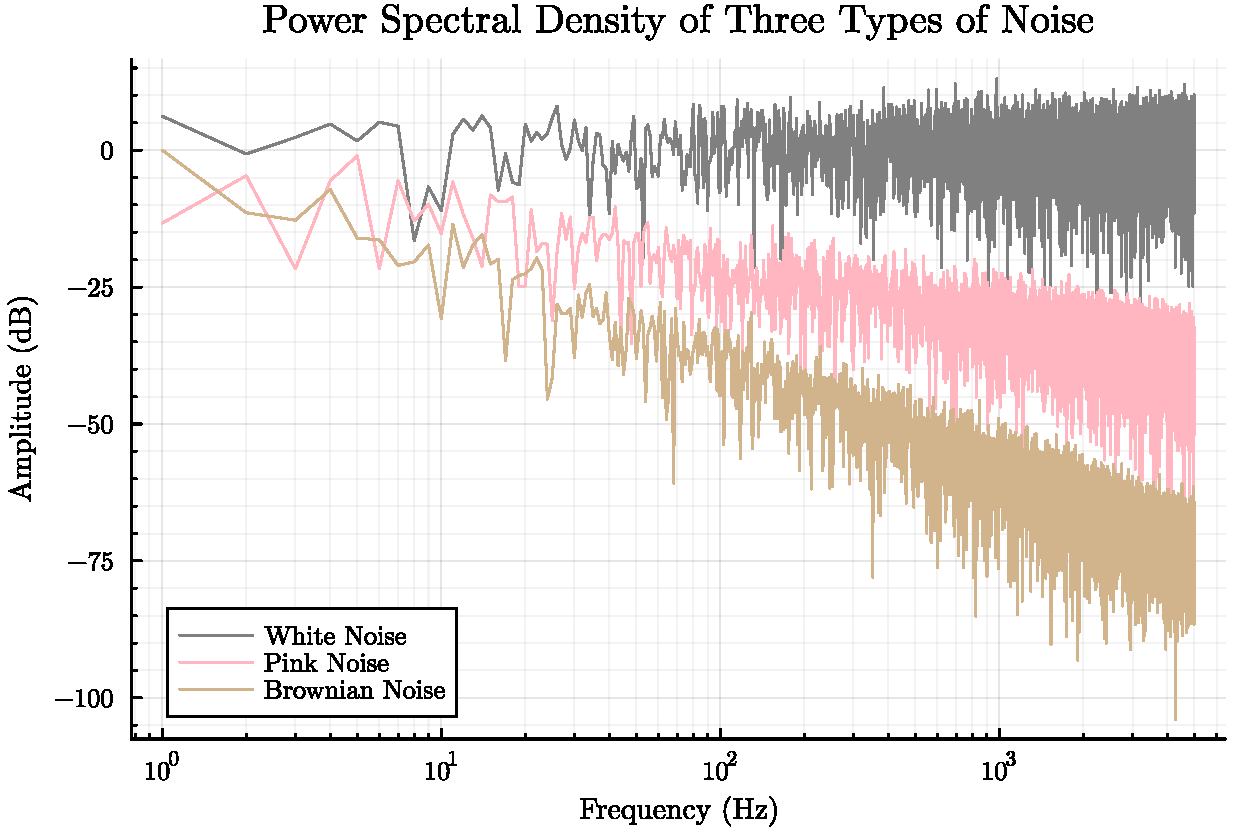
\includegraphics[scale = 0.6]{images/Background/Colors_of_noise.pdf}
                \caption{Power spectral densities of three types of noise. White noise is identifiable by a 0 slope on a logarithmic x-axis, where Brownian noise is identifiable by a -20dB/decade slope, and pink noise contains a slope of -10dB/decade slope.}
                %\noindent\makebox[\linewidth]{\rule{0.9\paperwidth}{0.4pt}}
            \end{figure}

        \subsection{Signal-to-Noise Ratio \& Weak Signals} \label{ss:weak_signals}
            Signal-to-Noise Ratio (SNR) is a widely used measurement for determining the quality of a signal. There are many definitions based on the type of signal being processed, however the most common is the ratio of powers definition.

            \begin{equation}
                SNR = \frac{P_s}{P_n}
            \end{equation}
            
            Where $P_s$ is the power of the signal and $P_n$ is the power of the noise. The signal power over a time period $T$ with $N$ samples can be defined as the absolute squares of the signal normalized by the signal length \cite{de_sousa_battery-resistor_2018}.

            \begin{equation} \label{power_eq}
                P = \frac{1}{N} \sum_{i=1}^{N} A_i^2
            \end{equation}

            where A denotes the amplitude of the signal. The power of the noise can be found by subtracting out the signal from the entire data set and then using equation \ref*{power_eq}. For measuring data without a signal present, the noise power is the preferred metric. 
            
            It is common practice to define SNR in terms of decibels because of the broad scales that the ratio can take \cite{sherman_transducers_2007}. The value of the SNR in dB is found by taking the logarithm of base 10 of the ratio of powers and multiplying by 10 \cite{kassam_robust_1985}.

            \begin{equation} \label{SNR_db_eq}
                SNR = 10log(\frac{P_s}{P_n})
            \end{equation}

            The decibel definition of the SNR approaches 0 dB as the value of the ratio of signal to noise power approaches unity. Because of the definition of signal power, signals with short periods or small amplitudes can have relatively low SNR values. 
            
            Most applications require high SNR, for example wireless networks recommend a SNR upwards of 25dB for streaming any sort of audio and video \cite{cisco_systems_signal--noise_2023}. However the benchmark for a weak signal is far below that at around the 0dB point \cite{wang_current_2013}. In the context of this thesis, only signals with negative decibel SNR values will be explored. 
            
        \subsection{Correlation Algorithms} \label{ss:correlations}
            The correlation is a classic form of feature detection algorithm in discrete signal processing and is often a component of a more complicated techniques. Correlations are a form of moving average processes and takes two classic forms in the autocorrelation and the cross-correlation. Broadly, we are able to define the autocorrelation function as the auto-covariance of the signal divided by the sample variance \cite{hamilton_time_1994}. Autocorrelations measure the correlation between a data set and a delayed copy of itself as a function of the delay \cite{lin_selective_2008}. The delay is commonly known as the lags $\tau$. Moreover, the result of the autocorrelation function (ACF) will show the similarity of random variables and any repeated patterns in the data set. For finite-discrete data sets, the autocorrelation function is an estimate of the autocorrelation for a infinite and continuous set of data. The ACF for a discrete data set $x(t) \in \mathbb{R}^N$ is defined as
            
            \begin{equation} \label{eq:ACF}
                R_{xx}(\tau) = \frac{1}{N}\sum_{0}^{N-1} x(t)x(t+\tau)
            \end{equation}

            which is equivalent to the expected value of the signal with the time delayed version of itself.

            \[
                R_{xx}(\tau) = \mathbb{E}[x(t)x(t+\tau)]
            \]
            
            The autocorrelation is connected to the convolution and can be represented as the convolution of the data with its time-reversed version. Convolution in the time domain can be represented as multiplication in the frequency domain by the convolution theorem \cite{harris_use_1978}. Thus the ACF can be represented in the Fourier domain. This vastly speeds up operation time having an $\mathbb{O}(Nlog(N))$ time dependency versus $\mathbb{O}(N^2)$ in the time domain.

            \begin{equation} \label{eq:f_acf}
                {R}_{xx}(\tau) = F^{-1}\{X(\omega) \odot X^*(\omega)\}
            \end{equation}
            
            Where $X(\omega)$ is the frequency domain representation of $x(t)$ and the complex conjugate of $X(\omega)$ is denoted by the star. ${R}_{xx}(\tau=0)$ is equivalent to the expected value of the power of the signal. The above definition in equation \ref*{eq:f_acf} is the non-normalized of the ACF. Normalization in the frequency domain is difficult to represent and often increases complexity. 
            
            Autocorrelations provide use in noise rejection from data, assuming stochastic noise. The larger the number of data points $N$ the more accurate the ACF will be and the better the noise rejection. This takes advantage of random content's tendency to trend to an expected value of 0 as the set becomes infinitely large.

            \begin{figure} [h]
                \centering
                \begin{subfigure}[c]{0.49\textwidth}
                    \centering
                    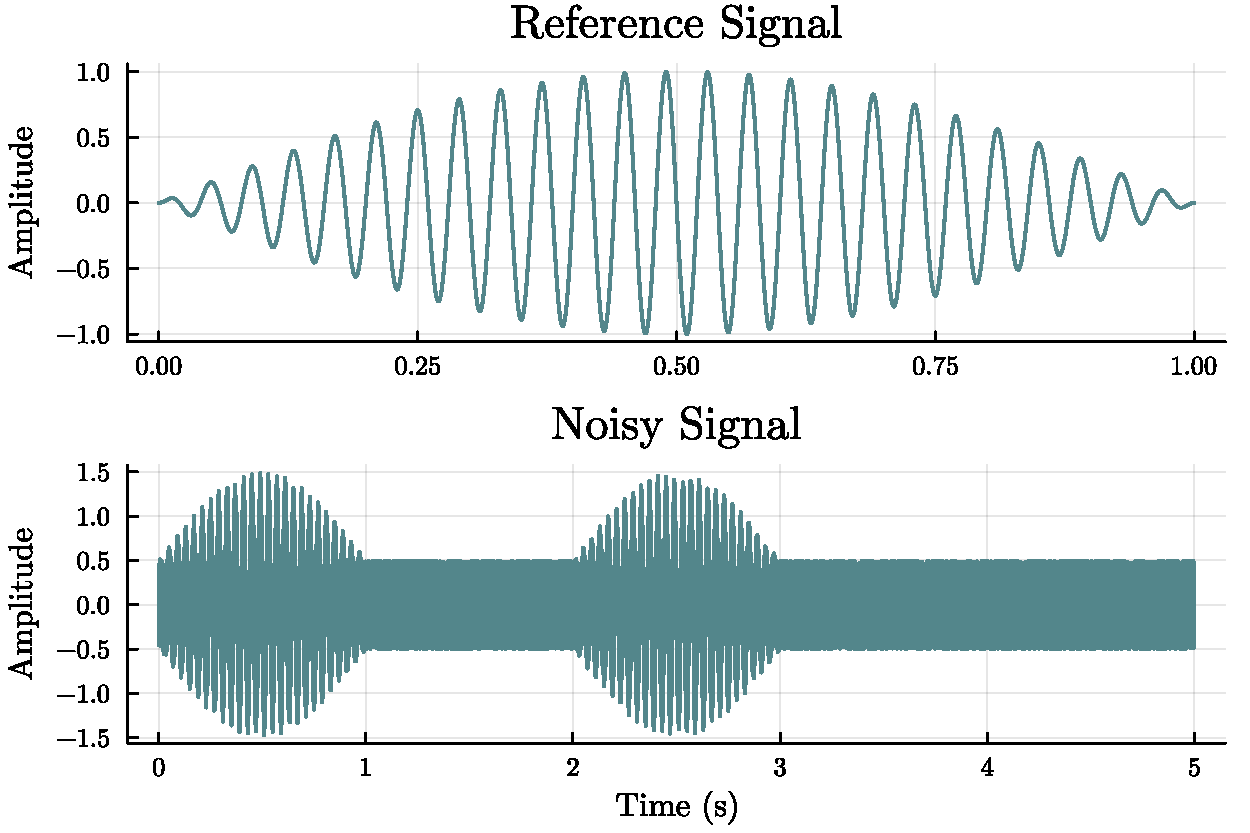
\includegraphics[width=\textwidth]{images/Background/Auto Correlation Reference and Data.pdf}
                    \caption{Original signal with roughly 0dB SNR}
                    \label{fig: original signal autocorr}
                \end{subfigure}
                \hfill
                \begin{subfigure}[c]{0.49\textwidth}
                    \centering
                    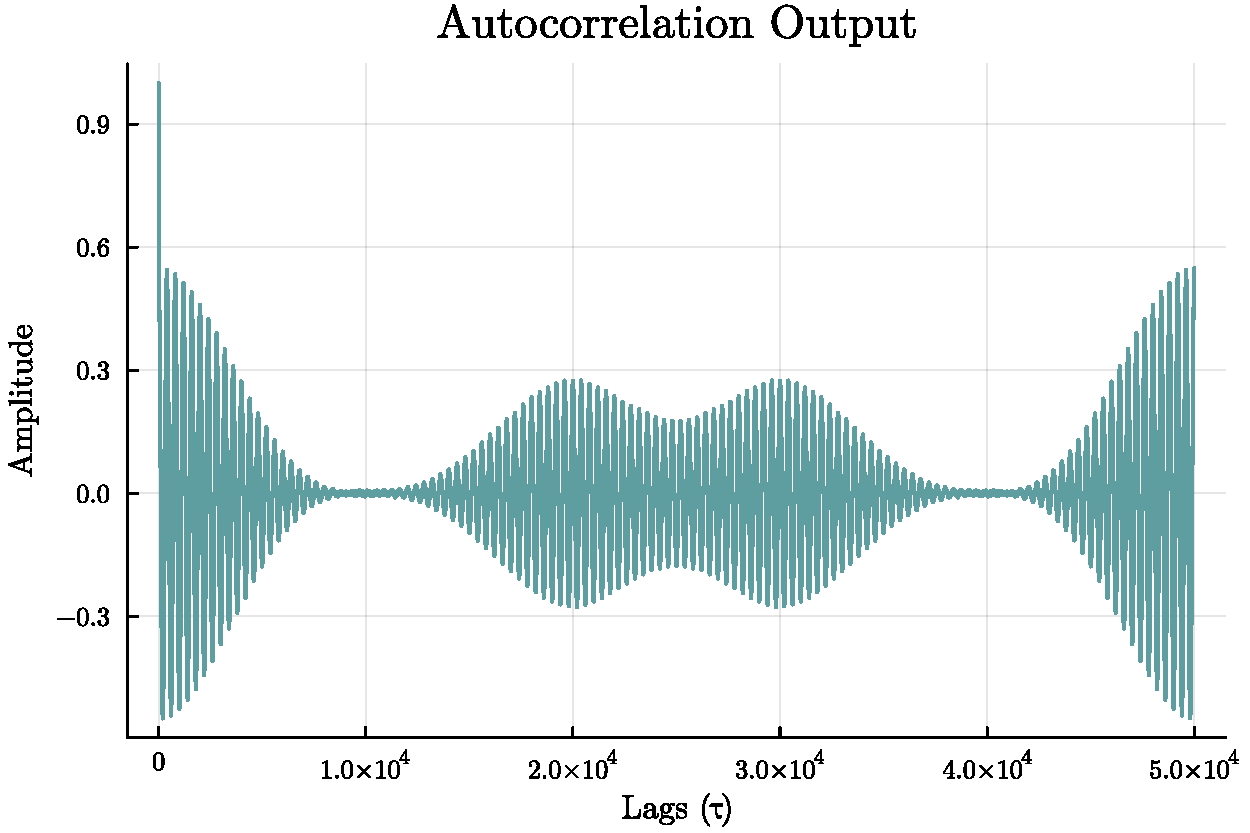
\includegraphics[width=\textwidth]{images/Background/AutoCorrelation Output.pdf}
                    \caption{Autocorrelation output}
                    \label{fig:autocorr out}
                \end{subfigure}
                \hfill
                \caption{Given an original noisy signal like that of the signal in (a), the autocorrelation output (b) describes the location of repeated events in the signals. The two-sided autocorrelation centered at 0 is shown. The local maxima appears at $\tau = 3$ indicating that a repeated event has occurred starting at that location.}
                \label{fig:example autocorr}
            \end{figure} 
            
            Where the autocorrelation uses a time delayed version of the original signal, the cross-correlation uses a time delayed reference signal $y(t) \in \mathbb{R}^N$. The cross-correlation is used to check for similarities to $y(t)$ within $x(t)$.
            
            \begin{equation} \label{eq:XCF}
                {R}_{xy}(\tau) = \frac{1}{N} \sum_{0}^{N-1} x(t)y(t+\tau)
            \end{equation}
            
            Similarly to the autocorrelation, the cross-correlation for the finite data set is an estimator for the continuous-infinite cross-correlation. The cross-correlation ${R}_{xy}(\tau=0)$ will be the same as the expected value of the convolution of the two signals reversed. Similarly to the autocorrelation, the cross-correlation can be represented as an expected value of the two data sets \cite{smith_mathematics_2007}. 
            
            \[
                R_{xy}(\tau) = \mathbb{E}[x(t)y(t+\tau)]
            \]
            
            The cross-correlation also has a frequency domain representation as was proved for equation \ref{eq:f_acf}. This can be found by performing element-wise multiplication of the Fourier transform of the original data and the complex conjugate of the frequency domain of the reference signal \cite{hamilton_time_1994}\cite{harris_use_1978}. 

            \begin{equation} \label{eq:f_xcf}
                {R}_{xy}(\tau) = F^{-1}\{X(\omega) \odot Y^*(\omega)\}
            \end{equation}

            In equation \ref*{eq:f_xcf}, $F^{-1}$ denotes the inverse Fast Fourier Transform (FFT) operator, $Y^*(\omega)$ denotes the complex conjugate of $y(t)$ in the frequency domain, and $\odot$ represents element wise multiplication. The use of this principle can be used to drastically speed up calculations for correlation functions of large data sets. In the frequency domain, the XCF follows $\mathbb{O}(Nlog(N))$ complexity as the samples size increases, the same as the autocorrelation. The normalized version of the correlation in the frequency domain takes a much more complicated form and is difficult to calculate because of the transformation of the normalization term into the frequency domain. 

            The time domain definition of the cross-correlation will yield an output of length $2*N - 1$. The frequency domain definition will have a length of $N$ because of the element wise definition of multiplication. Therefore, in both domains, the signals $x(t)$ and $y(t)$ must contain the same number of discrete data points.

            The benefit of the cross correlation function is its usage in template matching within data. By checking against a reference, the local maxima within the resultant correlation are the points wherein the original signal $x_j$ best matches the selected reference set $y_j$.

            \begin{figure} [h]
                \centering
                \begin{subfigure}[b]{0.45\textwidth}
                    \centering
                    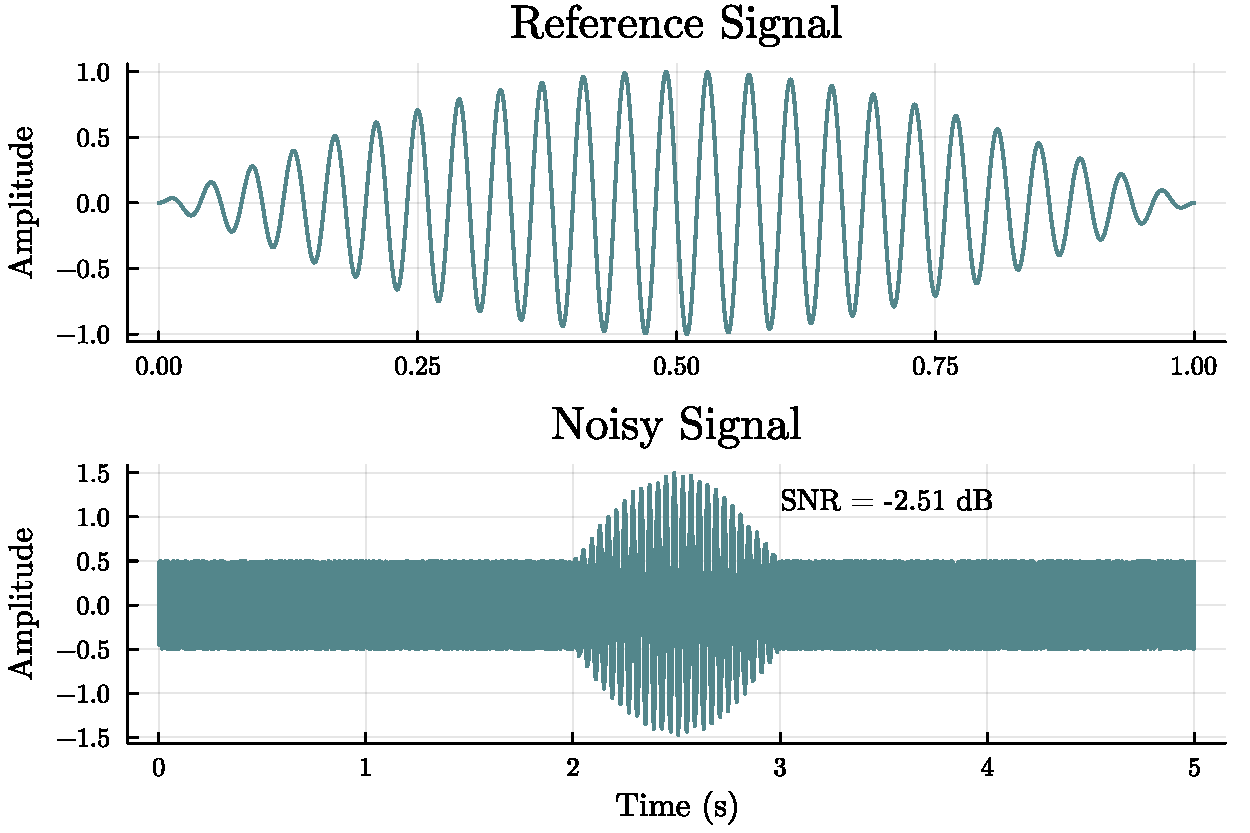
\includegraphics[width=\textwidth]{images/Background/Cross Correlation Reference and Data.pdf}
                    \caption{Original signal and reference signal}
                    \label{fig: original and ref}
                \end{subfigure}
                \hfill
                \begin{subfigure}[b]{0.45\textwidth}
                    \centering
                    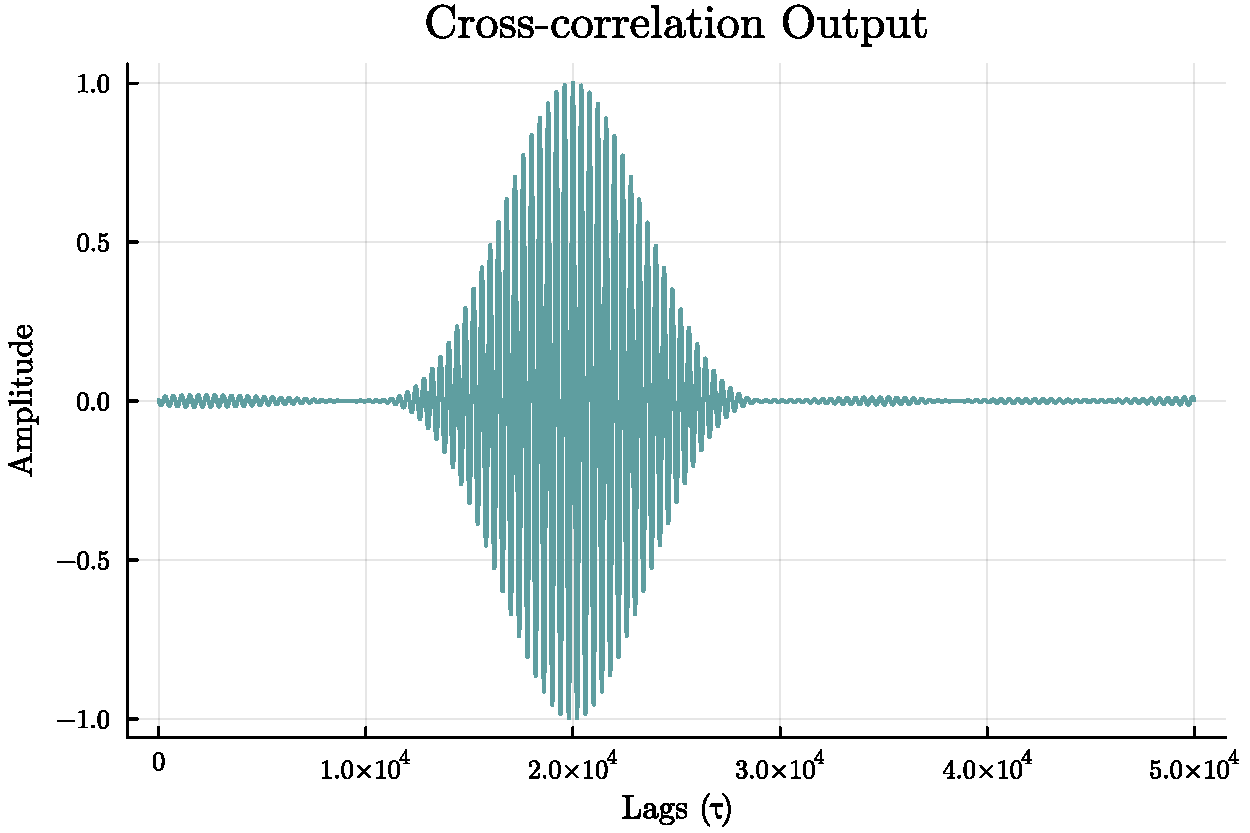
\includegraphics[width=\textwidth]{images/Background/Cross Correlation Output.pdf}
                    \caption{Cross-correlation output}
                    \label{fig:xcorr out}
                \end{subfigure}
                \hfill
                \caption{Simple example case of a cross-correlation of a sinusoidal signal with white noise. The correlation local maxima occur at where the beginning of the reference pulse lines up with the beginning of the sine pulse. In this case, those locations would be at $\tau = 0$ and $\tau = 3$.}
                \label{fig:example 1}
            \end{figure} 

            Cross-correlations have been adapted into other formats, particularly for array noise rejection, known as a cross-channel correlation algorithm. The cross-channel correlation can observe similarities between $p$ number of channels and remove redundant information. The correlated data is assumed to be noise and the remaining parts of the signal are considered "new" information \cite{michels_multichannel_1995}. Multi-channel cross correlations have found use in beam forming applications where the uncorrelated channels are deemed to have incoherent data and are thus considered unreliable \cite{kumatani_channel_2011}.

            The cross-correlation's ability to detect patterns in data are not just used in a signal time-history context. The sizes of $x(t)$ and $y(t)$ can be any arbitrary size [$m$ x $n$] so long as both have the same size. This is another benefit of the frequency domain representation. Therefore, the correlation can be used to calculate similarities between two images, known as template matching. 
            
            This style of cross-correlation is mathematically very similar to the single dimensional case. For this application, the normalized version of the cross-correlation is more accurate and thus preferred. In this case the use of the frequency domain convolution theorem is still used, however the normalization term of is reduced to an integral of search area image and image squared approach. The computation requirements for the image correlations thus evolve at a rate of $\mathbb{O}(3N^2)$ as opposed to $\mathbb{O}(3N^2(M-N + 1)^2)$ \cite{lewis_fast_1995}. Modern applications of the cross-correlation include face verification algorithms and feature detection in computer vision systems \cite{savvides_face_nodate} \cite{kumar_correlation_2006} \cite{hsu_correlation-based_2018}. 

            \begin{figure} [h]
                \centering
                \begin{subfigure}[c]{0.45\textwidth}
                    \centering
                    \includegraphics[width=\textwidth]{images/Background/Image Template Matching Example.jpg}
                    \caption{Original image, reference image used for template matching, and cross-correlation output}
                    \label{fig: template matching 1}
                \end{subfigure}
                \hfill
                \begin{subfigure}[c]{0.45\textwidth}
                    \centering
                    \includegraphics[width=\textwidth]{images/Background/Image Template Matching Example Output.jpg}
                    \caption{Original Image with box placed around location where template matching identified presence of the reference image}
                    \label{fig:template match out}
                \end{subfigure}
                \hfill
                \caption{A simple example case of an image cross-correlation example for template matching able to detect the bouquet of tulips within the original photo using fast normalized cross-correlator proposed by Lewis \cite{lewis_fast_1995}.}
                \label{fig:template match example}
                %\noindent\makebox[\linewidth]{\rule{0.9\paperwidth}{0.4pt}}
            \end{figure}


        \subsection{Correlations as Building Blocks} \label{ss:corr building blocks}

            The correlation algorithm can be used as the building blocks for other signal processing algorithms. The power spectral density (PSD), or autospectrum, is defined as the Fourier Transform of the autocorrelation by the Wiener-Khinchin theorem. If the discrete Fast Fourier Transform is defined as 

            \[
                S(\omega) = \sum_{j=0}^{N - 1}f_j(x)e^{-i\omega t j/N}
            \]
            
            then the discrete-time PSD can be written as
            
            \begin{equation}
                S(\omega) = \sum_{j=0}^{N-1}R_{xx}(\tau)e^{-i\omega t j/N}
            \end{equation}

            where $R_{xx}(\tau)$ is the definition of the autocorrelation as given by equation \ref{eq:ACF}. By expansion of the definition of the autocorrelation function $R_{xx}(\tau)$, the formula for the PSD becomes, the Fourier transform of the convolution of the signal with the time reversed version of itself. 

            \[
                S(\omega) = \sum_{j=0}^{N-1} \sum_{j=0}^{N} (x_j) (x_{j+\tau}) e^{-i\omega t j/N}
            \]

            \[
                S(\omega) = \sum_{j=0}^{N-1} \mathbb{E}[x(t)x(t-\tau)] e^{-i\omega t j/N}
            \]

            Applying the convolution theorem \cite{harris_use_1978} to the definition of the autocorrelation, $\mathbb{E}[x(t)x(t-\tau)]$ can be expressed as the inverse Fourier Transform of the multiplication of the frequency domain expression of the data set $\hat{X}(\omega)$ and its complex conjugate.

            \[
                S(\omega) = \sum_{j=0}^{N-1} \sum_{j=0}^{N - 1} {X}(\omega) \odot {X}^*(\omega)e^{i\omega t j/N}  e^{-i\omega t j/N}
            \]

            The Fourier transform and the inverse Fourier Transform can be cancelled and the PSD takes the form of the absolute value of the element wise multiplication in the frequency domain \cite{smith_mathematics_2007}.

            \begin{equation} \label{eq:PSD}
                S_{xx}(\omega) = |X(\omega) \odot X^*(\omega)|
            \end{equation}

            Mathematically the autospectrum is very similar to the frequency domain definition of the autocorrelation, the difference being the expression is left in the frequency domain.

            The use of the autospectrum is widespread and has applications in neurophysics research as well as tracking climate patterns \cite{wen_separating_2016} \cite{storch_statistical_1999}. In terms of signal detection, the PSD can help identify the most powerful frequency components within a noisy signal. This has limitations and typically requires a high SNR to work properly.
            
            The cross-spectrum is similar to the autospectrum, in that it is the frequency domain decomposition of the cross-correlation \cite{smith_mathematics_2007}. The cross-spectral density of a signal can be found in a similar manner to the cross-correlation definition in equation \ref{eq:f_xcf}, and is defined as absolute value of the data in frequency domain, times the complex conjugate of the reference \cite{racz_multiple-resampling_2022}. Like the cross-correlation, the cross-spectrum evolves at an $O(Nlog(N))$ time complexity.

            \begin{equation} \label{eq:CSD}
                S_{xy}(\omega) = |X(\omega) \odot Y^*(\omega)|
            \end{equation}

            The cross-spectrum is used to show the power of the shared frequency content between two signals and is commonly used to identify the frequencies present of data in a system. The cross-spectrum was created as an alternative to other frequency decomposition algorithms as the cross-spectrum is able to accurately measure the frequencies of short time, low signal-to-noise ratio (SNR) signals. Cross-spectral analysis is also quick comparative to other frequency decomposition methods of signals \cite{liu_optimization_2022}.

            \begin{figure} [h]
                \centering
                \begin{subfigure}[c]{0.48\textwidth}
                    \centering
                    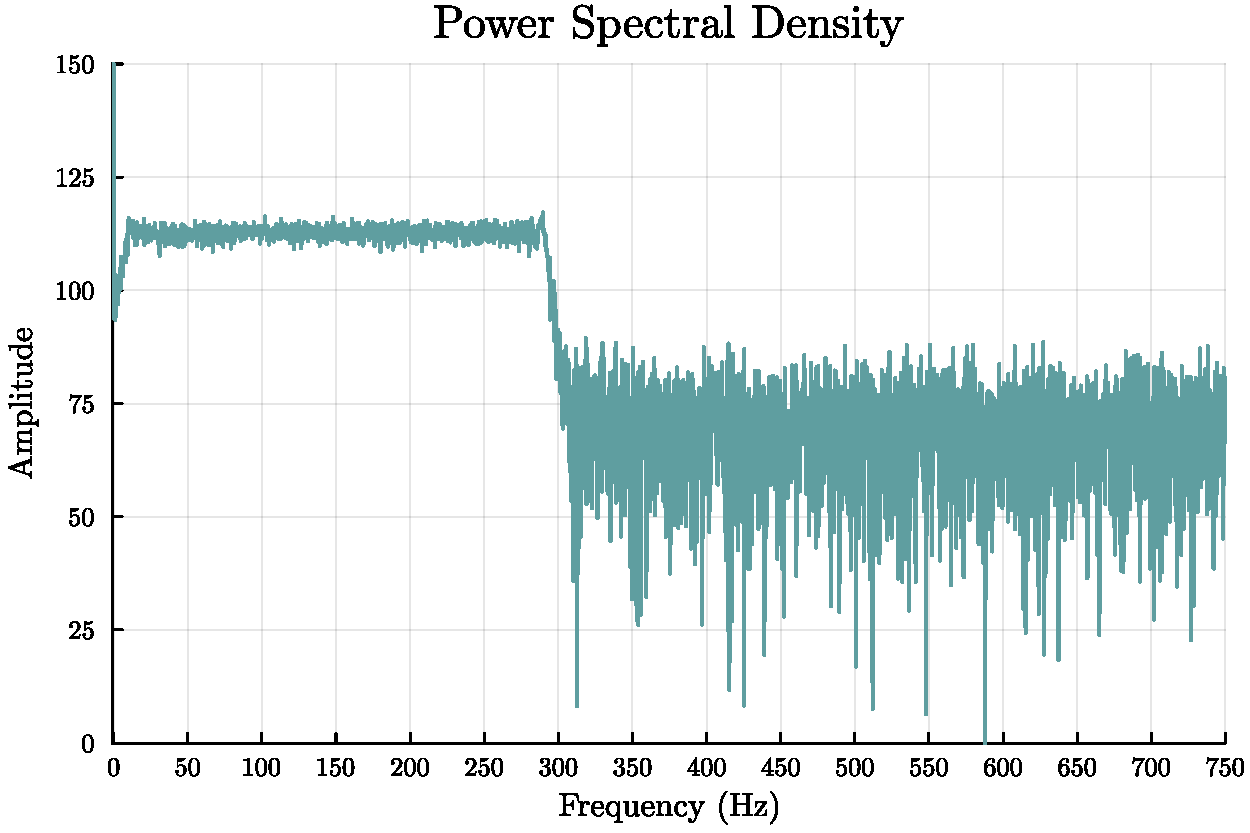
\includegraphics[width=\textwidth]{images/Background/Power Spectral Density.pdf}
                    \caption{Power Spectral Density of a linear swept frequency cosine (chirp) from 10 to 300 Hz}
                    \label{fig:PSD Example}
                \end{subfigure}
                \hfill
                \begin{subfigure}[c]{0.49\textwidth}
                    \centering
                    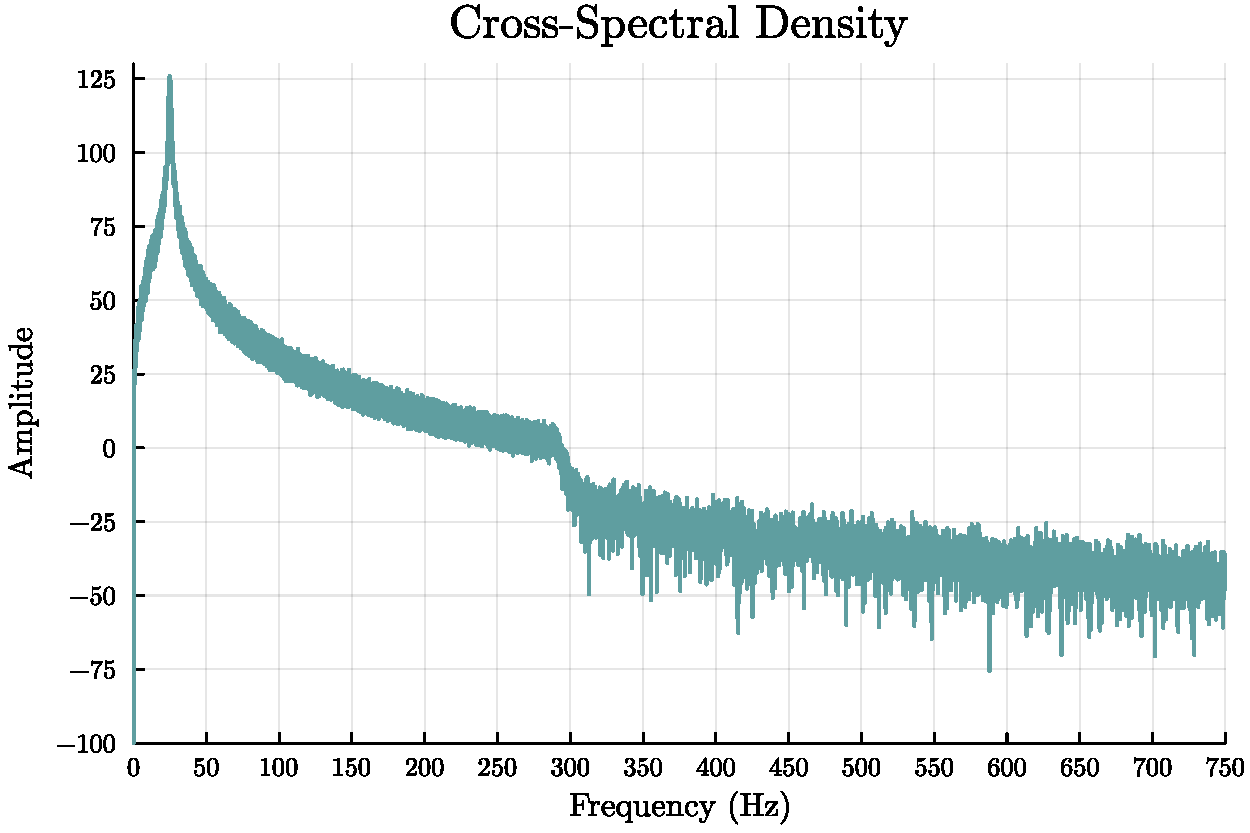
\includegraphics[width=\textwidth]{images/Background/Cross Spectral Density.pdf}
                    \caption{Cross-spectral density of a chirp signal in noise using a sine wave of 25 Hz as reference}
                    \label{fig:CSD Example}
                \end{subfigure}
                \hfill
                \caption{Power spectral density of a chirp from 10-300 Hz in (a) has a sharp drop off at 300 Hz indicating a signal is present in the data. The cross-spectrum shown in (b) where the data from (a) is checked against a sine wave of 25 Hz for the presence of shared frequencies. The peak appears at the expected shared frequency strongly indicating presence of a deterministic signal.}
                \label{fig:CSD and PSD}
            \end{figure}

        \subsection{Matched Filtering}
            Filtering data is a common method to reduce additive noise present in a signal. The standard linear filter is the convolution of the data with a windowing function that can reject unwanted frequencies that do not carry data. In short, filtering acts as a partial suppression of components of a signal. 

            Digital filters can be used for signal detection, but are more optimized for noise rejection, whereas a matched filter is the preferred digital filter for signal detection. Matched filters are optimum linear digital filters used for optimizing the SNR of a signal in the presence of stochastic additive noise. Matched filters are commonly used in radar and sonar systems as well as digital communications.

            A comprehensive derivation of the matched filter can be found using the Schwarz's inequality to maximize output signal energy to noise energy in received signal \cite{ziemer_principles_2015}. Assuming the noise is stationary, the theorem holds and any signal $s(t)$ with additive noise $n(t)$ has a filter that is matched to its impulse response

            \begin{equation} \label{eq:matched_filter}
                h(t) = g(T - t)
            \end{equation}

            where $g$ is an arbitrary constant and $T$ is the filter output time. Equation \ref*{eq:matched_filter} implies the maximum SNR is achieved when this filter has an impulse response that is the same as the complex conjugate, time-reversed input signal \cite{bancroft_introduction_2002}. The transfer function of the matched filter corresponds to the complex conjugate of the spectrum of the received signal $s(t)$ \cite{turin_introduction_1960}. 

            \begin{equation}
                H(\omega) = gS^*(\omega)e^{-j\omega T}
            \end{equation}

            
        \subsection{Time-Frequency Distributions} \label{ss:TFD}
            Often, our data stored in signals may change their frequency with time, these are non-stationary signals. Standard Fourier analyses are able to describe the frequency versus intensity relationship in our data, however it fails to relate to variations of the data in time domain. Time frequency distributions (TFD) are a powerful signal processing technique used to analyze the spectral content of our data by decomposing it into time, frequency, and intensity \cite{gabor_theory_1946} \cite{hamilton_time_1994}. Thus allowing relationships to be made between the three. 

            The most simple of the time frequency distribution algorithms is the is the Spectrogram, which makes use of the Short-Time-Fourier-Transform (STFT). The STFT makes use of windowing the data over certain time intervals and using the signal power over that window to determine the frequency relationship to time. Sliding the window over the entire data set can give a temporal resolution to the frequency content that is contained in the data \cite{cohen_time-frequency_1989}. This describes the intensity per unit frequency for each time step window. 

            \begin{equation}
                S(\tau, \omega) = \frac{1}{\sqrt{2\pi}} \int_{\tau = 0}^T s(t) h(\tau - t) e^{(j\omega\tau)} \,d\tau
            \end{equation}

            This is the continuous version of the STFT, which can be discretized and squared to quantify the power of each unit frequency in time within the signal \cite{cohen_time-frequency_1989} \cite{sejdic_timefrequency_2009}. 

            \begin{equation}
                S(\tau, \omega) = [\frac{1}{\sqrt{2\pi}} \sum_{\tau = 0}^T s(t) h(\tau - mt) e^{(j\omega\tau)}]^2
            \end{equation}

            The function of $h(\tau -mt)$ is the windowing function of the spectrogram and is responsible for the temporal resolution. There are many choices of windowing function that are used for different reasons \cite{varanis_comparison_2020} \cite{harris_use_1978}. Ultimately the windowing is the largest flaw of the spectrogram as it is unable to capture short frequencies that occur within one window, and there is limited control over the size variation with respect to frequency \cite{sejdic_timefrequency_2009}. When this occurs signal may be drowned out by surrounding spectra which dominates the time window.

            Where the spectrogram fails, the Wigner distribution succeeds in calculating high resolution time-frequency distributions. The Wigner-Ville distribution (WVD) is a modern TFD that is used to estimate signals with incredibly short time periods and instantaneous frequency estimations \cite{boashash_use_1993}. The Wigner-Ville distribution generalizes a relationship to the PSD through the use of autocorrelation \cite{varanis_comparison_2020} \cite{claasen_wigner_1980}. 

            \begin{equation} \label{eq:WVD_x}
                W_{x}(\tau, \omega) = 2\sum_{j=-N}^{N} e^{-i2j\omega}x(\tau +j) x^*(\tau - j)
            \end{equation}

            Where equation \ref*{eq:WVD_x} is the Wigner-Ville distribution in its canonical discrete form \cite{kumar_wigner-ville_2022} \cite{haykin_wigner-ville_1994}. For signal detection, and instantaneous frequency estimation of non-stationary signals, the cross Wigner-Ville distribution may also used due to its ability to handle noise at much lower SNR values \cite{guanghua_wigner-ville_2006}. 

            \begin{equation} \label{eq:XWVD}
                 W_{xy}(\tau, \omega) = 2\sum_{j=-N}^{N} e^{-i2j\omega}x(\tau +j) y^*(\tau - j)
            \end{equation}

            \begin{figure} [t]
                \centering
                \begin{subfigure}[c]{0.45\textwidth}
                    \centering
                    \includegraphics[width=\textwidth]{images/Background/Spectrogram Example.jpg}
                    \caption{Spectrogram}
                    \label{fig: spectrogram 1}
                \end{subfigure}
                \hfill
                \begin{subfigure}[c]{0.45\textwidth}
                    \centering
                    \includegraphics[width=\textwidth]{images/Background/WVD Example.jpg}
                    \caption{Wigner-Ville distribution}
                    \label{fig: WVD 1}
                \end{subfigure}
                \hfill
                \caption{A simple example case of a spectrogram (a) and Wigner-Ville distribution (b) of a logarithmic chirp from 300 Hz to 4 kHz. The width of the spectrogram appears much thicker than the width of the Wigner-Ville distribution, and will detect shorter period signals because of the higher resolution scale.}
                \label{fig:wvd and spectrogram}
            \end{figure}
        
            \nomenclature{STFT}{Short-Time-Fourier-Transform} 
            \nomenclature{TFD}{Time-Frequency Distribution}
            \nomenclature{WVD}{Wigner-Ville Distribution}
            \nomenclature{$\tau$}{The time delay of a correlation algorithm. Is referred to as lags and is a function of the sample rate of a signal where the max lag of a correlation will be $2N-1$.} 
            \nomenclature{ACF}{Abbreviation for the autocorrelation function.}
            \nomenclature{PSD}{Power Spectral Density, the frequency decomposition of the autocorrelation of a signal. }
            \nomenclature{XCF}{Abbreviation for the cross-correlation function.}
            \nomenclature{FFT}{Fast Fourier Transform}
            \nomenclature{SNR}{Signal-to-Noise Ratio}

            